\documentclass[titlepage,a4paper,12pt,oneside,dvipdfmx]{jsbook}
\usepackage[dvipdfmx]{graphicx}
\usepackage{amsmath,amssymb}
\usepackage{mathrsfs}
\usepackage{amsthm}
\usepackage{booktabs}
\usepackage{bm}
\usepackage{plext}
\usepackage{color} 
\usepackage{here}
%\usepackage{slashbox}
\usepackage{comment}

%\usepackage{emathUtf}
%\usepackage{subfigure}
%\usepackage[subrefformat=parens]{subcaption}
\newtheorem{theorem}{定理}
\renewcommand{\figurename}{Fig.}
\renewcommand{\tablename}{Table }
\setlength{\textheight}{20cm}
\setlength{\textwidth}{13.5cm}
%\setlength{\textheight}{22cm}
%\setlength{\textwidth}{15cm}

\setlength{\marginparwidth}{1.5cm}


	\setlength{\topmargin}{40pt}
	\iftombow
 	\addtolentgh{\topmargin}{-1in}
	\else
 	\addtolength{\topmargin}{-1truein}
	\fi

\setlength{\oddsidemargin}{0.0cm}
\setlength{\evensidemargin}{0.0cm}

\begin{document}

\chapter{トポロジー導関数の導出}
\section{固有振動モードの変動に関する方程式}

\begin{figure}[ht]
	\begin{center}
		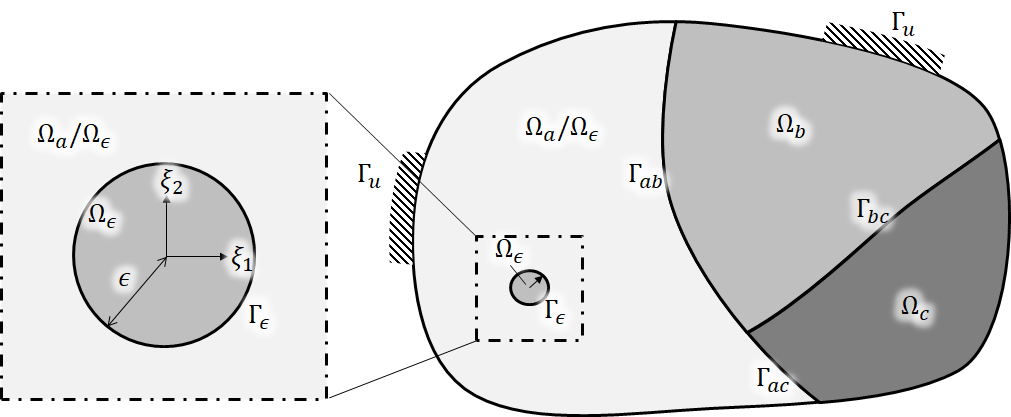
\includegraphics[width=13cm]{./figures/TD.png}
		\caption{Topological derivative}
		\label{fig:TD}
	\end{center}
\end{figure}

固有振動モードの変動$\hat{\bm{u}}(\bm{\xi})$に関する支配方程式は以下のようになる.
\begin{align}
&C_{ijkl}^{b} \hat{w}^{(-)}_{k,lj}(\bm{\xi})
+\epsilon^2\{(\lambda+\hat{\lambda})\rho^{b} \hat{w}_{i}^{(-)}(\bm{\xi})\}=0&&\text{in}\hspace{0.3cm}\Omega_{\epsilon}
\label{eq:GovDisturIn}
\\
&C_{ijkl}^{a}\hat{w}^{(+)}_{k,lj}(\bm{\xi})
+\epsilon^2\Bigl \{\lambda\rho^{a} \hat{w}_{i}^{(+)}(\bm{\xi})
+\hat{\lambda}\rho^{a} \bigl(u_{i}^{}(\bm{x})+\hat{w}_{i}^{(+)}(\bm{\xi}) \bigr) \Bigr \}=0
&&\text{in}\hspace{0.3cm}\Omega\backslash\Omega_{\epsilon}
\label{eq:GovDisturOut}
\\
&\hat{w}_{i}^{(-)}(\bm{\xi})-\hat{w}_{i}^{(+)}(\bm{\xi})=u_{i}(\bm{x})=u_{i}(\bm{x_0})+\epsilon \xi_j u_{i,j}(\bm{x_0})+O(\epsilon^2)
&&\text{on}\hspace{0.3cm}\Gamma_{\epsilon}
\label{eq:GovDisturUBC}
\\
&C_{ijkl}^{b}\hat{w}_{k,l}^{(-)}(\bm{\xi})n_{j}^{(-)}
-C_{ijkl}^{a}\hat{w}_{k,l}^{(+)}(\bm{\xi})n_{j}^{(-)}
=\epsilon C_{ijkl}^{a}u_{k,l}(\bm{x_0})n_{j}^{(-)}+O(\epsilon^2)
&&\text{on}\hspace{0.3cm}\Gamma_{\epsilon}
\label{eq:GovDisturSBC}
\\
&\sum_{p=1}^{n}\int_{\Omega_p}\rho^{p}(2u_{i}\hat{w}_{i}^{(+)}+\hat{w}_{i}^{(+)}\hat{w}_{i}^{(+)}) d\Omega
+\int_{\Omega_{\epsilon}}\{\rho^{b}\hat{w}_{i}^{(-)}\hat{w}_{i}^{(-)}-\rho^{a}u_{i}u_{i}\} d\Omega=0
\label{eq:GovDisturNorm}
\\
&\hat{w}_{i}^{(+)}(\bm{\xi})\rightarrow 0 \hspace{0.3cm} (|\bm{\xi}|\rightarrow \infty)
\label{eq:GovDisturInftyBC}
\end{align}

$\epsilon$の0次の項を整理すると
\begin{align}
&C_{ijkl}^{b} \hat{w}^{(I-)}_{k,lj}(\bm{\xi})=0&\text{in}\hspace{0.3cm}\Omega_{\epsilon}
\label{eq:GovDisturIn1}
\\
&C_{ijkl}^{a} \hat{w}^{(I+)}_{k,lj}(\bm{\xi})=0&\text{in}\hspace{0.3cm}\Omega\backslash\Omega_{\epsilon}
\label{eq:GovDisturOut1}
\\
&\hat{w}_{i}^{(I-)}(\bm{\xi})-\hat{w}_{i}^{(I+)}(\bm{\xi})=u_{i}(\bm{x_0}) &\text{on}\hspace{0.3cm}\Gamma_{\epsilon}
\label{eq:GovDisturUBC1}
\\
&C_{ijkl}^{b}\hat{w}_{k,l}^{(I-)}(\bm{\xi})n_{j}^{(-)}
-C_{ijkl}^{a}\hat{w}_{k,l}^{(I+)}(\bm{\xi})n_{j}^{(-)}=0 &\text{on}\hspace{0.3cm}\Gamma_{\epsilon}
\label{eq:GovDisturSBC1}
\\
&\hat{w}_{i}^{(I+)}(\bm{\xi})\rightarrow 0 \hspace{0.3cm} (|\bm{\xi}|\rightarrow \infty)
\label{eq:GovDisturInftyBC1}
\end{align}

$\epsilon$の1次の項を整理すると
\begin{align}
&C_{ijkl}^{b} \hat{w}^{(I\hspace{-.15em}I-)}_{k,lj}(\bm{\xi})=0
&\text{in}\hspace{0.3cm}\Omega_{\epsilon}
\label{eq:GovDisturIn2}
\\
&C_{ijkl}^{a} \hat{w}^{(I\hspace{-.15em}I+)}_{k,lj}(\bm{\xi})=0
&\text{in}\hspace{0.3cm}\Omega\backslash\Omega_{\epsilon}
\label{eq:GovDisturOut2}
\\
&\hat{w}_{i}^{(I\hspace{-.15em}I-)}(\bm{\xi})
-\hat{w}_{i}^{(I\hspace{-.15em}I+)}(\bm{\xi})= \xi_j u_{i,j}(\bm{x_0})=u_{i}^{(I\hspace{-.15em}I)} &\text{on}\hspace{0.3cm}\Gamma_{\epsilon}
\label{eq:GovDisturUBC2}
\\
&C_{ijkl}^{b}\hat{w}_{k,l}^{(I\hspace{-.15em}I-)}(\bm{\xi})n_{j}^{(-)}
-C_{ijkl}^{a}\hat{w}_{k,l}^{(I\hspace{-.15em}I+)}(\bm{\xi})n_{j}^{(-)}
=C_{ijkl}^{a} u_{k,l}^{}(\bm{x_0})n_{j}^{(-)}=t_{i}^{(I\hspace{-.15em}I)} &\text{on}\hspace{0.3cm}\Gamma_{\epsilon}
\label{eq:GovDisturSBC2}
\\
&\hat{w}_{i}^{(I\hspace{-.15em}I+)}(\bm{\xi})\rightarrow 0 \hspace{0.3cm} (|\bm{\xi}|\rightarrow \infty)
\label{eq:GovDisturInftyBC2}
\end{align}
以上から,$\hat{\bm{u}}^{(I-)}$,$\hat{\bm{u}}^{(I+)}$,$\hat{\bm{u}}^{(I\hspace{-.15em}I-)}$,$\hat{\bm{u}}^{(I\hspace{-.15em}I+)}$は,それぞれ平衡方程式に従うことが分かる.

\newpage

\section{等方弾性体の平衡方程式の一般解}

応力が$x_{3}$成分に依存しない場合の平衡方程式は以下のようになる.
\begin{align}
	\frac{\partial \sigma_{x_{1}x_{1}}}{\partial x_{1}}+\frac{\partial \sigma_{x_{1}x_{2}}}{\partial x_{2}}=0,\hspace{1cm}
	\frac{\partial \sigma_{x_{1}x_{2}}}{\partial x_{1}}+\frac{\partial \sigma_{x_{2}x_{2}}}{\partial x_{2}}=0
	\label{eq:2dequilibrium}
\end{align}
あるスカラー関数$\Phi$を用いて,応力テンソルの各成分を次式で表現することができれば,その応力は明らかに平衡方程式\eqref{eq:2dequilibrium}を満たす.
\begin{align}
	\sigma_{x_{1}x_{1}}=\frac{\partial^2 \Phi}{\partial x_{2}^2},\hspace{1cm}
	\sigma_{x_{2}x_{2}}=\frac{\partial^2 \Phi}{\partial x_{1}^2},\hspace{1cm}
	\sigma_{x_{1}x_{2}}=-\frac{\partial^2 \Phi}{\partial x_{1} \partial x_{2}}
	\label{eq:Airyxy}
\end{align}
このスカラー関数$\Phi$はThe Airy stress functionと呼ばれる.
弾性体を解析するには平衡条件に加えて適合条件を満たす必要がある.適合条件とは,
弾性体の複数の点の相対的な位置関係が変形によって変化しないことを保証する条件で,二次元の場合には歪みを用いて次式で与えられる.
\begin{align}
	\frac{\partial^2 e_{x_{1}x_{1}}}{\partial^2 x_{2}}
	-2\frac{\partial^2 e_{x_{1}x_{2}}}{\partial x_{1} \partial x_{2}}
	+\frac{\partial^2 e_{x_{2}x_{2}}}{\partial^2 x_{1}}
	\label{eq:Compatibility}
\end{align}
また,等方弾性体の場合,ひずみと応力の関係式は以下で表される.
\begin{align}
	\sigma_{ij}&=C_{ijkl}^{}e_{kl}^{}
	\nonumber
	\\
	C_{ijkl}&=\frac{3-\kappa}{\kappa-1}\mu\delta_{ij}\delta_{kl}
	+\mu(\delta_{ik}\delta_{jl}+\delta_{il}\delta_{jk})
	\label{eq:Constitute}
\end{align}
ただし,$\mu$は$\mu=\dsp\frac{E}{2(1+\nu)}$で与えられるラメ定数,
$\kappa$はKolosov's constantと呼ばれる定数で,
平面応力状態では式\eqref{eq:PlainStress},平面ひずみ状態では式\eqref{eq:PlainStrain}となる.
\begin{align}
	\kappa&=\frac{3-\nu}{1+\nu}\hspace{1cm}\text{(for plain stress)}
	\label{eq:PlainStress}
	\\
	\kappa&=3-4\nu\hspace{0.9cm}\text{(for plain strain)}
	\label{eq:PlainStrain}
\end{align}
ここで,式\eqref{eq:Airyxy}および\eqref{eq:Constitute}から,ひずみ$e_{ij}$を$\Phi$で表現すると次式のようになる.
\begin{align}
	e_{x_{1}x_{1}}=\frac{\kappa+1}{8\mu}\sigma_{x_{1}x_{1}}-\frac{3-\kappa}{8\mu}\sigma_{x_{2}x_{2}}
	=\frac{\kappa+1}{8\mu}\frac{\partial^2 \Phi}{\partial x_{2}^2}-\frac{3-\kappa}{8\mu}\frac{\partial^2 \Phi}{\partial x_{1}^2}
	\nonumber
	\\
	e_{x_{2}x_{2}}=\frac{\kappa+1}{8\mu}\sigma_{x_{2}x_{2}}-\frac{3-\kappa}{8\mu}\sigma_{x_{1}x_{1}}
	=\frac{\kappa+1}{8\mu}\frac{\partial^2 \Phi}{\partial x_{1}^2}-\frac{3-\kappa}{8\mu}\frac{\partial^2 \Phi}{\partial x_{2}^2}
	\nonumber
	\\
	e_{x_{1}x_{2}}=\hspace{0.3cm}\frac{1}{2\mu}\sigma_{x_{1}x_{2}}\hspace{0.3cm}
	=-\frac{1}{2\mu}\frac{\partial^2 \Phi}{\partial x_{1} \partial x_{2}}\hspace{1.5cm}
	\label{eq:DefPhi}
\end{align}
式\eqref{eq:Compatibility}に\eqref{eq:DefPhi}を代入し,整理すると次式が得られる.
\begin{align}
	\nabla^4\Phi=0
	\label{eq:biharmonic}
\end{align}
ゆえに$\Phi$は重調和関数となる.

二次元の極座標系において,式\eqref{eq:biharmonic}にはThe Michell solutionと呼ばれる一般解が存在し,$\Phi$は以下のように展開される.
\begin{align}
	\Phi =&A_{01}r^2+A_{02}r^2\ln(r)+A_{03}\ln(r)+A_{04}\theta
	\nonumber
	\\
	&+\Bigl(A_{11}r^3+A_{12}r\ln(r)+A_{14}r^{-1}\Bigr)\cos(\theta)+A_{13}r\theta\sin(\theta)
	\nonumber
	\\
	&+\Bigl(B_{11}r^3+B_{12}r\ln(r)+B_{14}r^{-1}\Bigr)\sin(\theta)+B_{13}r\theta\cos(\theta)
	\nonumber
	\\
	&+\sum_{m=2}^{\infty}\Bigl(A_{m1}r^{m+2}+A_{m2}r^{-m+2}
	+A_{m3}r^{m}+A_{m4}r^{-m}\Bigr)\cos(m\theta)
	\nonumber
	\\
	&+\sum_{m=2}^{\infty}\Bigl(B_{m1}r^{m+2}+B_{m2}r^{-m+2}
	+B_{m3}r^{m}+B_{m4}r^{-m}\Bigr)\sin(m\theta)
	\label{eq:Michell}
\end{align}

極座標表示における,応力テンソルの各成分$\sigma_{rr},\sigma_{r\theta},\sigma_{\theta\theta}$はThe Airy stress function $\Phi$を用いて次式で表現される.
\begin{align}
	\sigma_{rr}=\frac{1}{r}\frac{\partial \Phi}{\partial r}
	+\frac{1}{r^2}\frac{\partial^2 \Phi}{\partial \theta^2},\hspace{1cm}
	\sigma_{r\theta}=\frac{1}{r^2}\frac{\partial \Phi}{\partial \theta}
	-\frac{1}{r}\frac{\partial^2 \Phi}{\partial r\partial \theta},\hspace{1cm}
	\sigma_{\theta\theta}=\frac{\partial^2 \Phi}{\partial r^2}
	\label{eq:Airyrtheta}
\end{align}
ゆえに,式\eqref{eq:Airyrtheta}に式\eqref{eq:Michell}を代入すると,$\sigma_{rr},\sigma_{r\theta},\sigma_{\theta\theta}$は次式のようになる.
\begin{align}
	\sigma_{rr} =&2A_{01}
	+A_{02}\bigl\{ 2r\ln(r)+1\bigr\}
	+A_{03}r^{-2}
	\nonumber
	\\
	&+2A_{11}r\cos(\theta)
	+A_{12}r^{-1}\cos(\theta)
	+2A_{13}r^{-1}\cos(\theta)
	-2A_{14}r^{-3}\cos(\theta)
	\nonumber
	\\
	&+2B_{11}r\sin(\theta)
	+B_{12}r^{-1}\sin(\theta)
	-2B_{13}r^{-1}\sin(\theta)
	-2B_{14}r^{-3}\sin(\theta)
	\nonumber
	\\
	&+\sum_{m=2}^{\infty}\Bigl\{-A_{m1}(m+1)(m-2)r^{m}
	-A_{m2}(m+2)(m-1)r^{-m}
	\nonumber
	\\
	&\hspace{2.5cm}
	-A_{m3}m(m-1)r^{m-2}
	-A_{m4}m(m+1)r^{-m-2}\Bigr\}\cos(m\theta)
	\nonumber
	\\
	&+\sum_{m=2}^{\infty}\Bigl\{-B_{m1}(m+1)(m-2)r^{m}
	-B_{m2}(m+2)(m-1)r^{-m}
	\nonumber
	\\
	&\hspace{2.5cm}
	-B_{m3}m(m-1)r^{m-2}
	-B_{m4}m(m+1)r^{-m-2}\Bigr\}\sin(m\theta)
	\label{eq:SigmaRR}
\end{align}

\begin{align}
	\sigma_{r\theta} =&A_{04}r^{-2}
	\nonumber
	\\
	&+2A_{11}r\sin(\theta)
	+A_{12}r^{-1}\sin(\theta)
	-2A_{14}r^{-3}\sin(\theta)
	\nonumber
	\\
	&-2B_{11}r\cos(\theta)
	-B_{12}r^{-1}\cos(\theta)
	+2B_{14}r^{-3}\cos(\theta)
	\nonumber
	\\
	&+\sum_{m=2}^{\infty}\Bigl\{A_{m1}m(m+1)r^{m}
	-A_{m2}m(m-1)r^{-m}
	\nonumber
	\\
	&\hspace{1.5cm}
	+A_{m3}m(m-1)r^{m-2}
	-A_{m4}m(m+1)r^{-m-2}\Bigr\}\sin(m\theta)
	\nonumber
	\\
	&+\sum_{m=2}^{\infty}\Bigl\{-B_{m1}m(m+1)r^{m}
	+B_{m2}m(m-1)r^{-m}
	\nonumber
	\\
	&\hspace{1.5cm}
	-B_{m3}m(m-1)r^{m-2}
	+B_{m4}m(m+1)r^{-m-2}\Bigr\}\cos(m\theta)
	\label{eq:SigmaRTh}
\end{align}

\begin{align}
	\sigma_{\theta\theta} =&2A_{01}
	+A_{02}\bigl\{ 2r\ln(r)+3\bigr\}
	-A_{03}r^{-2}
	\nonumber
	\\
	&+6A_{11}r\cos(\theta)
	+A_{12}r^{-1}\cos(\theta)
	2A_{14}r^{-3}\cos(\theta)
	\nonumber
	\\
	&+6B_{11}r\sin(\theta)
	+B_{12}r^{-1}\sin(\theta)
	+2B_{14}r^{-3}\sin(\theta)
	\nonumber
	\\
	&+\sum_{m=2}^{\infty}\Bigl\{A_{m1}(m+1)(m+2)r^{m}
	+A_{m2}(m-1)(m-2)r^{-m}
	\nonumber
	\\
	&\hspace{2.0cm}
	+A_{m3}m(m-1)r^{m-2}
	+A_{m4}m(m+1)r^{-m-2}\Bigr\}\cos(m\theta)
	\nonumber
	\\
	&+\sum_{m=2}^{\infty}\Bigl\{B_{m1}(m+1)(m+2)r^{m}
	+B_{m2}(m-1)(m-2)r^{-m}
	\nonumber
	\\
	&\hspace{2.0cm}
	+B_{m3}m(m-1)r^{m-2}
	+B_{m4}m(m+1)r^{-m-2}\Bigr\}\sin(m\theta)
	\label{eq:SigmaThTh}
\end{align}
さらに極座標系の歪み-変位関係式は\eqref{eq:DefDisp}のようになる.
\begin{align}
	e_{rr}=\frac{\partial u_{r}}{\partial r},\hspace{1cm}
	e_{r\theta}=\frac{1}{2}\Bigl( \frac{1}{r}\frac{\partial u_{r}}{\partial \theta}
	+\frac{\partial u_{\theta}}{\partial r}-\frac{u_{\theta}}{r}\Bigr),\hspace{1cm}
	e_{\theta\theta}=\frac{1}{r}\frac{\partial u_{\theta}}{\partial \theta}+\frac{u_{r}}{r}
	\label{eq:DefDisp}
\end{align}
式\eqref{eq:SigmaRR}~式\eqref{eq:SigmaThTh},構成式\eqref{eq:Constitute},および歪み-変位関係式\eqref{eq:DefDisp}
を用いて$u_r$および$u_\theta$を求めると,以下のようになる.
\begin{align}
	2\mu u_{r} =&D_{1}\cos(\theta)+D_{2}\sin(\theta)
	\nonumber
	\\
	&+A_{01}(\kappa-1)r
	+A_{02}\Bigl\{ (\kappa-1)r\ln(r)-r\Bigr\}
	-A_{03}r^{-1}
	\nonumber
	\\
	&+A_{11}(\kappa-2)r^2\cos(\theta)
	+A_{12}\frac{1}{2}\Bigl\{ (\kappa+1)\theta\sin(\theta) -\cos(\theta)+(\kappa-1)\ln(r)\cos(\theta) \Bigr\}
	\nonumber
	\\
	&\hspace{0.5cm}+A_{13}\frac{1}{2}\Bigl\{ (\kappa-1)\theta\sin(\theta) -\cos(\theta)+(\kappa+1)\ln(r)\cos(\theta) \Bigr\}
	+A_{14}r^{-2}\cos(\theta)
	\nonumber
	\\
	&+B_{11}(\kappa-2)r^2\sin(\theta)
	+B_{12}\frac{1}{2}\Bigl\{ -(\kappa+1)\theta\cos(\theta) -\sin(\theta)+(\kappa-1)\ln(r)\sin(\theta) \Bigr\}
	\nonumber
	\\
	&\hspace{0.5cm}+B_{13}\frac{1}{2}\Bigl\{ (\kappa-1)\theta\cos(\theta) +\sin(\theta)-(\kappa+1)\ln(r)\sin(\theta) \Bigr\}
	+B_{14}r^{-2}\sin(\theta)
	\nonumber
	\\
	&+\sum_{m=2}^{\infty}\Bigl\{A_{m1}(\kappa-m-1)r^{m+1}
	+A_{m2}(\kappa+m-1)r^{-m+1}
	\nonumber
	\\
	&\hspace{3.8cm}
	-A_{m3}mr^{m-1}
	+A_{m4}mr^{-m-1}\Bigr\}\cos(m\theta)
	\nonumber
	\\
	&+\sum_{m=2}^{\infty}\Bigl\{B_{m1}(\kappa-m-1)r^{m+1}
	+B_{m2}(\kappa+m-1)r^{-m+1}
	\nonumber
	\\
	&\hspace{3.8cm}
	-B_{m3}mr^{m-1}
	+B_{m4}mr^{-m-1}\Bigr\}\sin(m\theta)
	\label{eq:UR}
\end{align}
\begin{align}
	2\mu u_{\theta} =&-D_{1}\sin(\theta)+D_{2}\cos(\theta)+D_{3}r
	\nonumber
	\\
	&+A_{02}(\kappa+1)r\theta
	-A_{04}r^{-1}
	\nonumber
	\\
	&+A_{11}(\kappa+2)r^2\sin(\theta)
	+A_{12}\frac{1}{2}\Bigl\{ (\kappa+1)\theta\cos(\theta) -\sin(\theta)-(\kappa-1)\ln(r)\sin(\theta) \Bigr\}
	\nonumber
	\\
	&\hspace{0.5cm}+A_{13}\frac{1}{2}\Bigl\{ (\kappa-1)\theta\cos(\theta) -\sin(\theta)-(\kappa+1)\ln(r)\sin(\theta) \Bigr\}
	+A_{14}r^{-2}\sin(\theta)
	\nonumber
	\\
	&-B_{11}(\kappa+2)r^2\cos(\theta)
	+B_{12}\frac{1}{2}\Bigl\{ (\kappa+1)\theta\sin(\theta) +\cos(\theta)+(\kappa-1)\ln(r)\cos(\theta) \Bigr\}
	\nonumber
	\\
	&\hspace{0.5cm}+B_{13}\frac{1}{2}\Bigl\{ -(\kappa-1)\theta\sin(\theta) -\cos(\theta)-(\kappa+1)\ln(r)\cos(\theta) \Bigr\}
	-B_{14}r^{-2}\cos(\theta)
	\nonumber
	\\
	&+\sum_{m=2}^{\infty}\Bigl\{A_{m1}(\kappa+m+1)r^{m+1}
	-A_{m2}(\kappa-m+1)r^{-m+1}
	\nonumber
	\\
	&\hspace{3.8cm}
	+A_{m3}mr^{m-1}
	-A_{m4}mr^{-m-1}\Bigr\}\sin(m\theta)
	\nonumber
	\\
	&+\sum_{m=2}^{\infty}\Bigl\{-B_{m1}(\kappa+m+1)r^{m+1}
	+B_{m2}(\kappa-m+1)r^{-m+1}
	\nonumber
	\\
	&\hspace{3.8cm}
	-B_{m3}mr^{m-1}
	-B_{m4}mr^{-m-1}\Bigr\}\cos(m\theta)
	\label{eq:UTh}
\end{align}
ただし,式\eqref{eq:UR}の$D_{1}\cos(\theta)+D_{2}\sin(\theta)$や
式\eqref{eq:UTh}の$-D_{1}\sin(\theta)+D_{2}\cos(\theta)+D_{3}r$は式\eqref{eq:DefDisp}を積分することで現れる不定積分の項である.
\newpage

\include{S3_1Inner}
\section{$\hat{\bm{w}}^{(I+)}$および$\hat{\sigma}^{(I+)}$のThe Michell solutionによる表現}

一方,$\Omega_{a}\backslash\Omega_\epsilon$におけるThe Airy stress function $\Phi^{(I+)}$に関しても同様に,
The Michell solutionを用いて以下のように展開できる.
\begin{align}
\Phi^{(I+)} =&A_{01}^{(I+)}r^2+A_{02}^{(I+)}r^2\ln(r)+A_{03}^{(I+)}\ln(r)+A_{04}^{(I+)}\theta
\nonumber
\\
&+\Bigl(A_{11}^{(I+)}r^3+A_{12}^{(I+)}r\ln(r)+A_{14}^{(I+)}r^{-1}\Bigr)\cos(\theta)+A_{13}^{(I+)}r\theta \sin(\theta)
\nonumber
\\
&+\Bigl(B_{11}^{(I+)}r^3+B_{12}^{(I+)}r\ln(r)+B_{14}^{(I+)}r^{-1}\Bigr)\sin(\theta)+B_{13}^{(I+)}r\theta \cos(\theta)
\nonumber
\\
&+\sum_{m=2}^{\infty}\Bigl(A_{m1}^{(I+)}r^{m+2}+A_{m2}^{(I+)}r^{-m+2}
+A_{m3}^{(I+)}r^{m}+A_{m4}^{(I+)}r^{-m}\Bigr)\cos(m\theta)
\nonumber
\\
&+\sum_{m=2}^{\infty}\Bigl(B_{m1}^{(I+)}r^{m+2}+B_{m2}^{(I+)}r^{-m+2}
+B_{m3}^{(I+)}r^{m}+B_{m4}^{(I+)}r^{-m}\Bigr)\sin(m\theta)
\label{eq:AiryOut1}
\end{align}

$r\rightarrow\infty$において,$|\hat{\bm{w}}^{(I+)}|\rightarrow0$となる条件は以下のようになる,
\begin{align}
D_{1}^{(I+)}=0,\hspace{1cm}
D_{2}^{(I+)}=0,\hspace{1cm}
D_{3}^{(I+)}=0&
\nonumber
\\
A_{01}^{(I+)}=0,\hspace{1cm}A_{02}^{(I+)}=0&
\nonumber
\\
A_{11}^{(I+)}=0,\hspace{1cm}A_{12}^{(I+)}=0,\hspace{1cm}A_{13}^{(I+)}=0&
\nonumber
\\
B_{11}^{(I+)}=0,\hspace{1cm}B_{12}^{(I+)}=0,\hspace{1cm}B_{13}^{(I+)}=0&
\nonumber
\\
A_{m1}^{(I+)}=0,\hspace{1cm}A_{m3}^{(I+)}=0&\hspace{1cm}(m\geq2)
\nonumber
\\
B_{m1}^{(I+)}=0,\hspace{1cm}B_{m3}^{(I+)}=0&\hspace{1cm}(m\geq2)
\label{eq:ConOut1}
\end{align}
ゆえに,式\eqref{eq:ConOut1}を用いて$\hat{w}_{r}^{(I+)},\hat{w}_{\theta}^{(I+)},\hat{\sigma}_{rr}^{(I+)},\hat{\sigma}_{r\theta}^{(I+)}$を整理すると,以下のようになる.
\begin{align}
	2\mu^{a}\hat{w}_{r}^{(I+)} =&-A_{03}^{(I+)}r^{-1}
	\nonumber
	\\
	&+A_{14}^{(I+)}r^{-2}\cos(\theta)
	+B_{14}^{(I+)}r^{-2}\sin(\theta)
	\nonumber
	\\
	&+\sum_{m=2}^{\infty}\Bigl\{A_{m2}^{(I+)}(\kappa^{a}+m-1)r^{-m+1}
	+A_{m4}^{(I+)}mr^{-m-1}\Bigr\}\cos(m\theta)
	\nonumber
	\\
	&+\sum_{m=2}^{\infty}\Bigl\{B_{m2}^{(I+)}(\kappa^{a}+m-1)r^{-m+1}
	+B_{m4}^{(I+)}mr^{-m-1}\Bigr\}\sin(m\theta)
	\label{eq:UROut1}
\end{align}
\begin{align}
	2\mu^{a}\hat{w}_{\theta}^{(I+)} =&-A_{04}^{(I+)}r^{-1}
	\nonumber
	\\
	&+A_{14}^{(I+)}r^{-2}\sin(\theta)
	-B_{14}^{(I+)}r^{-2}\cos(\theta)
	\nonumber
	\\
	&+\sum_{m=2}^{\infty}\Bigl\{-A_{m2}^{(I+)}(\kappa^{a}-m+1)r^{-m+1}
	+A_{m4}^{(I+)}mr^{-m-1}\Bigr\}\sin(m\theta)
	\nonumber
	\\
	&+\sum_{m=2}^{\infty}\Bigl\{B_{m2}^{(I+)}(\kappa^{a}-m+1)r^{-m+1}
	-B_{m4}^{(I+)}mr^{-m-1}\Bigr\}\cos(m\theta)
	\label{eq:UThOut1}
\end{align}
\begin{align}
	\hat{\sigma}_{rr}^{(I+)} =&A_{03}^{(I+)}r^{-2}
	\nonumber
	\\
	&-2A_{14}^{(I+)}r^{-3}\cos(\theta)
	-2B_{14}^{(I+)}r^{-3}\sin(\theta)
	\nonumber
	\\
	&+\sum_{m=2}^{\infty}\Bigl\{
	-A_{m2}^{(I+)}(m+2)(m-1)r^{-m}
	-A_{m4}^{(I+)}m(m+1)r^{-m-2}\Bigr\}\cos(m\theta)
	\nonumber
	\\
	&+\sum_{m=2}^{\infty}\Bigl\{
	-B_{m2}^{(I+)}(m+2)(m-1)r^{-m}
	-B_{m4}^{(I+)}m(m+1)r^{-m-2}\Bigr\}\sin(m\theta)
	\label{eq:SigmaRROut1}
\end{align}
\begin{align}
	\hat{\sigma}_{r\theta}^{(I+)} =&A_{04}^{(I+)}r^{-2}
	\nonumber
	\\
	&-2A_{14}^{(I+)}r^{-3}\sin(\theta)
	+2B_{14}^{(I+)}r^{-3}\cos(\theta)
	\nonumber
	\\
	&+\sum_{m=2}^{\infty}\Bigl\{
	-A_{m2}^{(I+)}m(m-1)r^{-m}
	-A_{m4}^{(I+)}m(m+1)r^{-m-2}\Bigr\}\cos(m\theta)
	\nonumber
	\\
	&+\sum_{m=2}^{\infty}\Bigl\{
	B_{m2}^{(I+)}m(m-1)r^{-m}
	+B_{m4}^{(I+)}m(m+1)r^{-m-2}\Bigr\}\sin(m\theta)
	\label{eq:SigmaRThOut1}
\end{align}

\newpage

%\include{S4_1Outer_Alt}
\section{$\Gamma_{\epsilon}$上の境界条件から得られる等式}

$D_{i}^{*(I-)},A_{ij}^{*(I-)},B_{ij}^{*(I-)},A_{ij}^{*(I+)},B_{ij}^{*(I+)}$を次式のように定義する.
\begin{align}
	D_{i}^{(I-)}=2\mu^{b}D_{i}^{*(I-)},\hspace{1cm}A_{ij}^{(I-)}=2\mu^{b}A_{ij}^{*(I-)},\hspace{1cm}
	B_{ij}^{(I-)}=2\mu^{b}B_{ij}^{*(I-)}&
	\nonumber
	\\
	A_{ij}^{(I+)}=2\mu^{a}A_{ij}^{*(I+)},\hspace{1cm}
	B_{ij}^{(I+)}=2\mu^{a}B_{ij}^{*(I+)}&
	\label{eq:ChangeCoef}
\end{align}

$\Gamma_{\epsilon}(r=1)$上の変位および応力ベクトルの境界条件\eqref{eq:GovDisturUBC1}\eqref{eq:GovDisturSBC1}より,次の4つの等式が得られる.
\begin{align}
	\hat{w}_{r}^{(I-)}-\hat{w}_{r}^{(I+)} =&A_{01}^{*(I-)}(\kappa^{b}-1)-\Bigl(-A_{03}^{*(I+)}\Bigr)
	\nonumber
	\\
	&+\Bigl\{D_{1}^{*(I-)}+A_{11}^{*(I-)}(\kappa^{b}-2)
	-\Bigl(A_{14}^{*(I+)}\Bigr)\Bigr\}\cos(\theta)
	\nonumber
	\\
	&+\Bigl\{D_{2}^{*(I-)}+B_{11}^{*(I-)}(\kappa^{b}-2)
	-\Bigl(B_{14}^{*(I+)}\Bigr)\Bigr\}\sin(\theta)
	\nonumber
	\\
	&+\sum_{m=2}^{\infty}\Bigl\{A_{m1}^{*(I-)}(\kappa^{b}-m-1)
	-A_{m3}^{*(I-)}m
	\nonumber
	\\
	&\hspace{1.0cm}-\Bigl(A_{m2}^{*(I+)}(\kappa^{a}+m-1)
	+A_{m4}^{*(I+)}m\Bigr)\Bigr\}\cos(m\theta)
	\nonumber
	\\
	&+\sum_{m=2}^{\infty}\Bigl\{B_{m1}^{*(I-)}(\kappa^{b}-m-1)
	-B_{m3}^{*(I-)}m
	\nonumber
	\\
	&\hspace{1.0cm}-\Bigl(B_{m2}^{*(I+)}(\kappa^{a}+m-1)
	+B_{m4}^{*(I+)}m\Bigr)\Bigr\}\sin(m\theta)
	\nonumber
	\\
	=&u_{r}(\bm{x_{0}})
	\nonumber
	\\
	=&u_{x}(\bm{x_{0}})\cos(\theta)+u_{y}(\bm{x_{0}})\sin(\theta)
	\label{eq:UR1eq}
\end{align}
\begin{align}
	\hat{w}_{\theta}^{(I-)}-\hat{w}_{\theta}^{(I+)} =&D_{3}^{*(I-)}-\Bigl(-A_{04}^{*(I+)}\Bigr)
	\nonumber
	\\
	&+\Bigl\{-D_{1}^{*(I-)}+A_{11}^{*(I-)}(\kappa^{b}+2)
	-\Bigl(A_{14}^{*(I+)}\Bigr)\Bigr\}\sin(\theta)
	\nonumber
	\\
	&+\Bigl\{D_{2}^{*(I-)}-B_{11}^{*(I-)}(\kappa^{b}+2)
	-\Bigl(-B_{14}^{*(I+)}\Bigr)\Bigr\}\cos(\theta)
	\nonumber
	\\
	&+\sum_{m=2}^{\infty}\Bigl\{A_{m1}^{*(I-)}(\kappa^{b}+m+1)
	+A_{m3}^{*(I-)}m
	\nonumber
	\\
	&\hspace{1.0cm}-\Bigl(-A_{m2}^{*(I+)}(\kappa^{a}-m+1)
	+A_{m4}^{*(I+)}m\Bigr)\Bigr\}\sin(m\theta)
	\nonumber
	\\
	&+\sum_{m=2}^{\infty}\Bigl\{-B_{m1}^{*(I-)}(\kappa^{b}+m+1)
	-B_{m3}^{*(I-)}m
	\nonumber
	\\
	&\hspace{1.0cm}-\Bigl(B_{m2}^{*(I+)}(\kappa^{a}-m+1)
	-B_{m4}^{*(I+)}m\Bigr)\Bigr\}\cos(m\theta)
	\nonumber
	\\
	=&u_{\theta}(\bm{x_{0}})
	\nonumber
	\\
	=&-u_{x}(\bm{x_{0}})\sin(\theta)+u_{y}(\bm{x_{0}})\cos(\theta)
	\label{eq:UTh1eq}
\end{align}
\begin{align}
	\hat{\sigma}_{rr}^{(I-)}-\hat{\sigma}_{rr}^{(I+)} =
	&2A_{01}^{(I-)}-\Bigl(A_{03}^{(I+)}\Bigr)
	\nonumber
	\\
	&+\Bigl\{2A_{11}^{(I-)}
	-\Bigl(-2A_{14}^{(I+)}\Bigr)\Bigr\}\cos(\theta)
	\nonumber
	\\
	&+\Bigl\{2B_{11}^{(I-)}
	-\Bigl(-2B_{14}^{(I+)}\Bigr)\Bigr\}\sin(\theta)
	\nonumber
	\\
	&+\sum_{m=2}^{\infty}\Bigl\{
	-A_{m1}^{(I-)}(m+1)(m-2)-A_{m3}^{(I-)}m(m-1)
	\nonumber
	\\
	&\hspace{1.0cm}-\Bigl(-A_{m2}^{(I+)}(m+2)(m-1)-A_{m4}^{(I+)}m(m+1)\Bigr)
	\Bigr\}\cos(m\theta)
	\nonumber
	\\
	&+\sum_{m=2}^{\infty}\Bigl\{
	-B_{m1}^{(I-)}(m+1)(m-2)-B_{m3}^{(I-)}m(m-1)
	\nonumber
	\\
	&\hspace{1.0cm}-\Bigl(-B_{m2}^{(I+)}(m+2)(m-1)-B_{m4}^{(I+)}m(m+1)\Bigr)
	\Bigr\}\sin(m\theta)
	\nonumber
	\\
	=&0
	\label{eq:SigmaRReq}
\end{align}
\begin{align}
	\hat{\sigma}_{r\theta}^{(I-)}-\hat{\sigma}_{r\theta}^{(I+)} =
	&-A_{04}^{(I+)}
	\nonumber
	\\
	&+\Bigl\{2A_{11}^{(I-)}
	-\Bigl(-2A_{14}^{(I+)}\Bigr)\Bigr\}\sin(\theta)
	\nonumber
	\\
	&+\Bigl\{-2B_{11}^{(I-)}
	-\Bigl(2B_{14}^{(I+)}\Bigr)\Bigr\}\cos(\theta)
	\nonumber
	\\
	&+\sum_{m=2}^{\infty}\Bigl\{
 	A_{m1}^{(I-)}m(m+1)+A_{m3}^{(I-)}m(m-1)
	\nonumber
	\\
	&\hspace{1.0cm}-\Bigl(-A_{m2}^{(I+)}m(m-1)-A_{m4}^{(I+)}m(m+1)\Bigr)
	\Bigr\}\sin(m\theta)
	\nonumber
	\\
	&+\sum_{m=2}^{\infty}\Bigl\{
	-B_{m1}^{(I-)}m(m+1)-B_{m3}^{(I-)}m(m-1)
	\nonumber
	\\
	&\hspace{1.0cm}-\Bigl(B_{m2}^{(I+)}m(m-1)+B_{m4}^{(I+)}m(m+1)\Bigr)
	\Bigr\}\cos(m\theta)
	\nonumber
	\\
	=&0
	\label{eq:SigmaRTh1eq}
\end{align}

\newpage
\section{The Michell solutionの係数に関する連立方程式}

任意の$0\leq\pi\leq2\pi$に対して\eqref{eq:UR1eq}~\eqref{eq:SigmaRTh1eq}が成立するためには
$1$,$\cos(m\theta)$,$\sin(m\theta)$$(m\geq1)$の係数が0である必要がある.ゆえに,次下の連立方程式が得られる.

1の係数:
\begin{align}
	\left(
	\begin{array}{cccc}
		{\dsp\frac{1}{2\mu^b}}& 0 & 0 & {\dsp\frac{1}{2\mu^a}} \\
		0 & {\dsp\frac{\kappa^b-1}{2\mu^b}} & {\dsp\frac{1}{2\mu^a}} & 0 \\
		0 & 4 & -2 & 0 \\
		0 & 0 & 0 & -2 \\
	\end{array}
	\right)
	\left(
	\begin{array}{c}
		D_{3}^{(I-)} \\
	 	A_{01}^{(I-)} \\
		A_{03}^{(I+)}\\
	 	A_{04}^{(I+)} \\
	\end{array}
	\right)
	=
	\left(
	\begin{array}{c}
		0 \\
	 	0 \\
		0 \\
	 	0 \\
	\end{array}
	\right)
\end{align}
$\cos(\theta),\sin(\theta)$の係数:
\begin{align}
	\left(
	\begin{array}{ccc}
		{\dsp\frac{1}{2\mu^b}}& {\dsp\frac{\kappa^b-2}{2\mu^b}} & {\dsp-\frac{1}{2\mu^a}} \\
		{\dsp-\frac{1}{2\mu^b}} & {\dsp\frac{\kappa^b+2}{2\mu^b}} & {\dsp-\frac{1}{2\mu^a}} \\
		0 & 4 & 4 \\
	\end{array}
	\right)
	\left(
	\begin{array}{c}
		D_{1}^{(I-)} \\
	 	A_{11}^{(I-)} \\
	 	A_{14}^{(I+)} \\
	\end{array}
	\right)
	=
	\left(
	\begin{array}{c}
		u_{x}(\bm{x_{0}}) \\
	 	-u_{x}(\bm{x_{0}}) \\
	 	0 \\
	\end{array}
	\right)
\end{align}
\begin{align}
	\left(
	\begin{array}{ccc}
		{\dsp\frac{1}{2\mu^b}}& {\dsp\frac{\kappa^b-2}{2\mu^b}} & {\dsp-\frac{1}{2\mu^a}} \\
		{\dsp\frac{1}{2\mu^b}} & {\dsp-\frac{\kappa^b+2}{2\mu^b}} & {\dsp\frac{1}{2\mu^a}} \\
		0 & -4 & -4 \\
	\end{array}
	\right)
	\left(
	\begin{array}{c}
		D_{2}^{(I-)} \\
	 	B_{11}^{(I-)} \\
	 	B_{14}^{(I+)} \\
	\end{array}
	\right)
	=
	\left(
	\begin{array}{c}
		u_{y}(\bm{x_{0}}) \\
	 	u_{y}(\bm{x_{0}}) \\
	 	0 \\
	\end{array}
	\right)
\end{align}
\newpage
$\cos(m\theta),\sin(m\theta)$の係数$(m\geq2)$:
\begin{align}
	\left(
	\begin{array}{cccc}
		{\dsp\frac{ \kappa^b-m-1}{2\mu^{b}}}& {\dsp-\frac{m}{2\mu^{b}}} &
		{\dsp-\frac{\kappa^a+m-1}{2\mu^{a}}} & {\dsp-\frac{m}{2\mu^{a}}} \\
		{\dsp\frac{\kappa^b+m+1}{2\mu^{b}}} & {\dsp\frac{m}{2\mu^{b}}} &
		{\dsp\frac{\kappa^a-m+1}{2\mu^{a}}} & {\dsp-\frac{m}{2\mu^{a}}} \\
		-(m+1)(m-2) & -m(m-1) & (m+2)(m-1) & m(m+1) \\
		m(m+1) & m(m-1) & m(m-1) & m(m+1)\\
	\end{array}
	\right)
	\left(
	\begin{array}{c}
		A_{m1}^{(I-)} \\
	 	A_{m3}^{(I-)} \\
		A_{m2}^{(I+)}\\
	 	A_{m4}^{(I+)} \\
	\end{array}
	\right)
	=
	\left(
	\begin{array}{c}
		0 \\
	 	0 \\
		0 \\
	 	0 \\
	\end{array}
	\right)
\end{align}
\begin{align}
	\left(
	\begin{array}{cccc}
		{\dsp\frac{ \kappa^b-m-1}{2\mu^{b}}}& {\dsp-\frac{m}{2\mu^{b}}} &
		{\dsp-\frac{\kappa^a+m-1}{2\mu^{a}}} & {\dsp-\frac{m}{2\mu^{a}}} \\
		{\dsp-\frac{\kappa^b+m+1}{2\mu^{b}}} & {\dsp-\frac{m}{2\mu^{b}}} &
		{\dsp-\frac{\kappa^a-m+1}{2\mu^{a}}} & {\dsp \frac{m}{2\mu^{a}}} \\
		-(m+1)(m-2) & -m(m-1) & (m+2)(m-1) & m(m+1) \\
		-m(m+1) & -m(m-1) & -m(m-1) & -m(m+1)\\
	\end{array}
	\right)
	\left(
	\begin{array}{c}
		B_{m1}^{(I-)} \\
	 	B_{m3}^{(I-)} \\
		B_{m2}^{(I+)}\\
	 	B_{m4}^{(I+)} \\
	\end{array}
	\right)
	=
	\left(
	\begin{array}{c}
		0 \\
	 	0 \\
		0 \\
	 	0 \\
	\end{array}
	\right)
\end{align}
これらの連立方程式を解くと,
\begin{align}
	D_{1}^{(I-)}=2\mu^{b}u_{x}(\bm{x_{0}}),\hspace{0.5cm}
	D_{2}^{(I-)}=2\mu^{b}u_{y}(\bm{x_{0}}),\hspace{0.5cm}D_{3}^{(I-)}=0
	\nonumber
	\\
	A_{ij}^{(I\pm)}=0,\hspace{0.5cm}
	B_{ij}^{(I\pm)}=0,\hspace{0.5cm}(i\geq0,1\leq j\leq4)
\end{align}
以上から,$\hat{\bm{w}}^{(I)}$は以下のように求まる.
\begin{align}
	\hat{w}_{r}^{(I-)}=u_{x}(\bm{x_{0}})\cos(\theta)+u_{y}(\bm{x_{0}})\sin(\theta)
	\nonumber
	\\
	\hat{w}_{\theta}^{(I-)}=-u_{x}(\bm{x_{0}})\sin(\theta)+u_{y}(\bm{x_{0}})\cos(\theta)
	\nonumber
	\\
	\hat{w}_{r}^{(I+)}=0,\hspace{1.0cm}\hat{w}_{\theta}^{(I+)}=0\hspace{1.0cm}
\end{align}

\newpage


\section{$\hat{\bm{u}}^{(I\hspace{-.15em}I-)}$の導出}

境界$\Gamma_{\epsilon}$上の極座標$(1,\theta)$における$\xi_1,\xi_2$座標は$(\xi_1,\xi_2)=(\cos(\theta),\sin(\theta))$,法線ベクトルの$\xi_1,\xi_2$成分は$(n_{\xi_1},n_{\xi_2})=(\cos(\theta),\sin(\theta))$である.ゆえに$\Gamma_\epsilon$上の境界条件\eqref{eq:GovDisturUBC2}における変位$\bm{u}^{(I\hspace{-.15em}I)}$の$\xi_1,\xi_2$成分は以下のようになる.
\begin{align}
	u_{\xi_1}^{(I\hspace{-.15em}I)}=&\xi_{j} u_{x_{1},j}(\bm{x_{0}})
	\nonumber
	\\
	=&u_{x_{1},x_{1}}(\bm{x_{0}})\cos(\theta)+u_{x_{1},x_{2}}(\bm{x_{0}})\sin(\theta)
	\\
	u_{\xi_2}^{(I\hspace{-.15em}I)}=
	&u_{x_{2},x_{1}}(\bm{x_{0}})\cos(\theta)+u_{x_{2},x_{2}}(\bm{x_{0}})\sin(\theta)
\end{align}
ゆえに,$\bm{u}^{(I\hspace{-.15em}I)}$の$r,\theta$方向成分は以下のようになる.
\begin{align}
	u_{r}^{(I\hspace{-.15em}I)}=
		&u_{\xi_1}^{(I\hspace{-.15em}I)}\cos(\theta)+u_{\xi_2}^{(I\hspace{-.15em}I)}\sin(\theta)
		\nonumber
		\\
		=&u_{x_{1},x_{1}}(\bm{x_{0}})\cos^2(\theta)+\bigl\{u_{x_{1},x_{2}}(\bm{x_{0}})
		+u_{x_{2},x_{1}}(\bm{x_{0}})\bigr\}\sin(\theta)\cos(\theta)
		+u_{x_{2},x_{2}}(\bm{x_{0}})\sin^2(\theta)
		\nonumber
		\\
		=&\frac{1}{2}\bigl\{u_{x_{1},x_{1}}(\bm{x_{0}})+u_{x_{2},x_{2}}(\bm{x_{0}})\bigr\}
		+\frac{1}{2}\bigl\{u_{x_{1},x_{1}}(\bm{x_{0}})-u_{x_{2},x_{2}}(\bm{x_{0}})\bigr\}\cos(2\theta)
		\nonumber
		\\
		&+\frac{1}{2}\bigl\{u_{x_{1},x_{2}}(\bm{x_{0}})+u_{x_{2},x_{1}}(\bm{x_{0}})\bigr\}\sin(2\theta)
		\\
	u_{\xi_2}^{(I\hspace{-.15em}I)}=
		&-u_{\xi_1}^{(I\hspace{-.15em}I)}\sin(\theta)+u_{\xi_2}^{(I\hspace{-.15em}I)}\cos(\theta)
		\nonumber
		\\
		=&-\bigl\{u_{x_{1},x_{1}}(\bm{x_{0}})-u_{x_{2},x_{2}}(\bm{x_{0}})\bigr\}\cos(\theta)\sin(\theta)
		-u_{x_{1},x_{2}}(\bm{x_{0}})\sin^2(\theta)+u_{x_{2},x_{1}}(\bm{x_{0}})\cos^2(\theta)
		\nonumber
		\\
		=&-\frac{1}{2}\bigl\{u_{x_{1},x_{2}}(\bm{x_{0}})-u_{x_{2},x_{1}}(\bm{x_{0}})\bigr\}
		+\frac{1}{2}\bigl\{u_{x_{1},x_{2}}(\bm{x_{0}})+u_{x_{2},x_{1}}(\bm{x_{0}})\bigr\}\cos(2\theta)
		\nonumber
		\\
		&-\frac{1}{2}\bigl\{u_{x_{1},x_{1}}(\bm{x_{0}})-u_{x_{2},x_{2}}(\bm{x_{0}})\bigr\}\sin(2\theta)
\end{align}

また,$\Gamma_\epsilon$上の境界条件\eqref{eq:GovDisturSBC2}における応力ベクトル$\bm{t}^{(I\hspace{-.15em}I)}$の$\xi_1,\xi_2$成分は以下のようになる.
\begin{align}
	t_{\xi_1}^{(I\hspace{-.15em}I)}=&C_{1jkl}^{a}u_{k,l}^{}(\bm{x_{0}})n_{j}
		\nonumber
		\\
		=&\mu^a\Bigl\{\frac{\kappa^a+1}{\kappa^a-1} u_{x_{1},x_{1}}(\bm{x_{0}})
		+\frac{3-\kappa^a}{\kappa^a-1} u_{x_{2},x_{2}}(\bm{x_{0}})\Bigr\}\cos(\theta)
		\nonumber
		\\
		&+\mu^a\bigl\{u_{x_{1},x_{2}}(\bm{x_{0}})+u_{x_{2},x_{1}}(\bm{x_{0}})\bigr\}\sin(\theta)
	\\
	t_{\xi_2}^{(I\hspace{-.15em}I)}=&C_{2jkl}^{a}u_{k,l}^{}(\bm{x_{0}})n_{j}
		\nonumber
		\\
		=&\mu^a \bigl\{u_{x_{1},x_{2}}(\bm{x_{0}})+u_{x_{2},x_{1}}(\bm{x_{0}})\bigr\}\cos(\theta)
		\nonumber
		\\
		&+\mu^a\Bigl\{ \frac{3-\kappa^a}{\kappa^a-1} u_{x_{1},x_{1}}(\bm{x_{0}})
		+\frac{\kappa^a+1}{\kappa^a-1} u_{x_{2},x_{2}}(\bm{x_{0}})\Bigr\}\sin(\theta)
\end{align}
ゆえに,$\bm{t}^{(I\hspace{-.15em}I)}$の$r,\theta$方向成分は以下のようになる.
\begin{align}
	t_{r}^{(I\hspace{-.15em}I)}
		=&t_{\xi_1}^{(I\hspace{-.15em}I)}\cos(\theta)+t_{\xi_2}^{(I\hspace{-.15em}I)}\sin(\theta)
			\nonumber
			\\
		=&\mu^a\Bigl\{\frac{\kappa^a+1}{\kappa^a-1} u_{x_{1},x_{1}}(\bm{x_{0}})
			+\frac{3-\kappa^a}{\kappa^a-1} u_{x_{2},x_{2}}(\bm{x_{0}})\Bigr\}\cos^2(\theta)
			\nonumber
			\\
			&+2\mu^a\bigl\{u_{x_{1},x_{2}}(\bm{x_{0}})
			+u_{x_{2},x_{1}}(\bm{x_{0}})\bigr\}\sin(\theta)\cos(\theta)
			\nonumber
			\\
			&+\mu^a\Bigl\{ \frac{3-\kappa^a}{\kappa^a-1} u_{x_{1},x_{1}}(\bm{x_{0}})
			+\frac{\kappa^a+1}{\kappa^a-1} u_{x_{2},x_{2}}(\bm{x_{0}})\Bigr\}\sin^2(\theta)
			\nonumber
			\\
		=&\frac{2\mu^a}{\kappa^a-1}\Bigl\{ u_{x_{1},x_{1}}(\bm{x_{0}})
			+ u_{x_{2},x_{2}}(\bm{x_{0}})\Bigr\}
			\nonumber
			\\
			&+\mu^a\bigl\{u_{x_{1},x_{2}}(\bm{x_{0}})
			+u_{x_{2},x_{1}}(\bm{x_{0}})\bigr\}\sin(2\theta)
			\nonumber
			\\
			&+\mu^a\Bigl\{ u_{x_{1},x_{1}}(\bm{x_{0}})
			+ u_{x_{2},x_{2}}(\bm{x_{0}})\Bigr\}\cos(2\theta)
			\\
	t_{\theta}^{(I\hspace{-.15em}I)}				
		=&-t_{\xi_1}^{(I\hspace{-.15em}I)}\sin(\theta)+t_{\xi_2}^{(I\hspace{-.15em}I)}\cos(\theta)
			\nonumber
			\\
		=&-2\mu^a \bigl\{u_{x_{1},x_{2}}(\bm{x_{0}})-u_{x_{2},x_{1}}(\bm{x_{0}})\bigr\}\cos(\theta)\sin(\theta)
			\nonumber
			\\
			&+\mu^a \bigl\{u_{x_{1},x_{2}}(\bm{x_{0}})+u_{x_{2},x_{1}}(\bm{x_{0}})\bigr\}
			\bigl(\cos^2(\theta)-\sin^2(\theta)\bigr)
			\nonumber
			\\
		=&-\mu^a \bigl\{u_{x_{1},x_{2}}(\bm{x_{0}})-u_{x_{2},x_{1}}(\bm{x_{0}})\bigr\}\sin(2\theta)
			\nonumber
			\\
			&+\mu^a \bigl\{u_{x_{1},x_{2}}(\bm{x_{0}})+u_{x_{2},x_{1}}(\bm{x_{0}})\bigr\}\cos(2\theta)
\end{align}


\end{document}

